\documentclass[10pt, a4paper]{article}
\usepackage[utf8]{inputenc}
\usepackage{amsmath}
\usepackage{amssymb}
\usepackage{amsthm}
\usepackage{parskip}
\usepackage{enumitem}
\usepackage{siunitx}
\usepackage{tikz}
\usepackage{pgfplots}
\usepackage{graphicx}
\graphicspath{ {./} }
\usetikzlibrary{arrows.meta}
\usetikzlibrary{angles,quotes}
\pgfplotsset{compat = newest}

\title{Física Contemporánea\\Resolución de Tarea 3}
\author{Vite Riveros Carlos Emilio\\ Romero De La Rosa Gabriela Michelle\\ 
        Fisher Bautista Emir Julián\\ López Gallegos Fátima}
\date{25 octubre del 2022}

\begin{document}
    \maketitle

    Problemas:
    \begin{enumerate}
        \item Haz un diagrama de cuerpo libre de un buque y discute el principio de
        Arquímedes. También haz el diagrama de cuerpo libre del péndulo doble
        (¡sin susto!).

        \item Demuestra que la fuerza gravitacional “de prepa”, $\vec{f}=m\vec{g}$ y la 
        fuerza de gravitacional Universal, $\vec{F}=mG\frac{M}{r^2}\hat{r}$, son la misma. 
        Evalúa para el caso de la Tierra (busca los valores de $M_{\text{Tierra}}$ y $R_{\text{Tierra}}$).

        \begin{center}
            $M_\oplus= 5.9722 \times 10^{24}\si{kg}$, $R_\oplus= 6371 \si{km}=6371000\si{m}$\\
            $F = G\frac{m M_\oplus}{(R_\oplus+h)^2}$

            Como la altura $h$ suele ser insignificante, podemos aproximar:\\
             $(R_\oplus+h)^2\approx R_\oplus^2$.

            $F = G\frac{M_\oplus}{R_\oplus^2}m$\\
            $F = (6.67408\times 10^{-11})\frac{5.9722\times 10^{24}}{6371000^2}m$\\
            $F = m(9.8199...)$, $\si{g}\approx9.81\frac{\si{m}}{\si{s^2}}$\\
            $F = mg$

        \end{center}

        \item Suponiendo que la Luna gira alrededor de la Tierra con un periodo de 27
        días, a una distancia de $3.8 \times 10^8 \si{m}$, calcular la masa de la Tierra.

        \item Considera un satélite terrestre que describe una órbita cuyo radio es $1.5$
        veces el radio de la Tierra. Considerando órbita circular, 1. Calcula su
        período, 2. si se quiere que esté geoestacionario (busca éste término), calcula
        la altura a la que debe estar sobre la superficie de la Tierra.
        
        \item Identifique qué tipo de cónica representa la ecuación polar:
        \begin{center}
            $r=\frac{3}{4-\cos\theta}$
        \end{center}
        Haga una gráfica de esta curva en papel polar, o con Mathematica.

        \item La distancia media de Marte al sol es $1.52$ veces la de la Tierra al sol.
        A partir de esto, calcule el número de años necesarios para que Marte
        complete una revolución en torno al Sol.

        \item Considere una distribución esférica uniforme de estrellas en una galaxia
        de masa total $M$ y radio $R_0$. Cierta estrella de masa $M_e$ a una distancia
        $r < R_0$ del centro se moverá bajo la acción de una fuerza central cuyo
        módulo depende de la distancia incluida dentro de la esfera de radio $r$. 1.
        ¿Cuál es la fuerza en r? 2. ¿Cuál es la velocidad de la estrella si ésta se
        mueve alrededor del centro en una órbita circular? Hint: Use la densidad $p=\frac{M}{V}$

        \begin{center}
            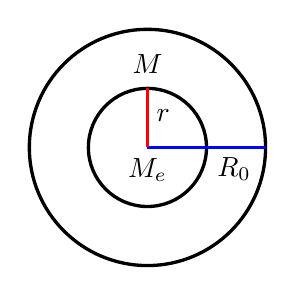
\begin{tikzpicture}
                \filldraw[very thick, fill=white] circle (1.5);
                \filldraw[very thick, fill=white] circle (.75) node[anchor=north]{$M_e$};
                \node[anchor=north] at (0, 1.3) {$M$};
                \draw[blue, thick] (0,0) -- (1.5,0);
                \draw[red, thick] (0,0) -- (0,.75);
                \node[anchor=north] at (1.1, 0) {$R_0$};
                \node[anchor=north] at (.2, .6) {$r$};
            \end{tikzpicture}

            1. $F=G\frac{M_e (M(r<))}{r^2}$, $p=\frac{M}{V}=\frac{M}{\frac{4}{3}\pi R_0^3}=\frac{M(r<)}{\frac{4}{3}\pi r^3}$\\ 
            $M(r<)=M(\frac{r}{R_0})^3$\\
            $F=G\frac{M_e M(\frac{r}{R_0})^3}{r^2}$\\
            $F=\frac{G M_e M r}{R_0^3}$

            2. $F_c=M_e\frac{V^2}{r}$, $Fc=\frac{G M_e M}{R_0^3}r$\\
            $M_e\frac{v^2}{r}=\frac{G M_e M}{R_0^3}r$\\
            $\frac{v^2}{r}=\frac{G M}{R_0^3}r$\\
            $v=\sqrt[]{\frac{GMr^2}{R_0^3}}$

        \end{center}
    \end{enumerate}

    Preguntas:
    \begin{enumerate}
        \item Si cayeras en un agujero perforado a través del centro de la Tierra y no
        intentaras sujetarte de los bordes al final, ¿Que clase de movimiento expe-
        rimentarías?

        \begin{center}
            Sería un movimiento oscilatorio, debido que al caer no hay nada que te detenga en el centro,
            continuas a través del agujero. Como no hay resistencia del aire, subes de nuevo a la superficie.
            Es decir, al no haber algo que te detenga, oscilarás de un lado a otro.
        \end{center}

        \item A la mitad del camino hacia el centro de la Tierra, ¿Pesarías más o menos
        que en la superficie?

        \begin{center}
            No es que pese menos, si no que en un punto, el centro de la tierra es donde las fuerzas
            gravitacionales provenientes de la masa que rodea este centro se contrarrestan entre sí.
            Así que en cierta forma pesarías menos.
        \end{center}

        \item ¿Por cuanto decrece la fuerza gravitacional entre dos objetos cuando la
        distancia entre ellos ¿se duplica? ¿se triplica?

        \begin{center}
            Cuando la distancia entre dos objetos aumenta, la fuerza disminuye como el cuadrado de 
            la distancia.
        \end{center}

    \end{enumerate}
\end{document}